\chapter{PREMIERS RÉSULTATS}
\thispagestyle{empty}

\section{Artefacts produits}

Le projet a déjà produit un ensemble substantiel de résultats concrets, et non
pas seulement quelques fragments de code préliminaires. Les artefacts les plus
importants sont les suivants :
\begin{itemize}
    \item le jeu de données expérimental Custom-WikiCS dérivé de Wiki-CS avec
    des champs textuels Wikipedia enrichis,
    \item des caches de plongements sémantiques fondés sur BGE-M3,
    \item des caches de plongements structurels pour plusieurs variantes de
    Node2Vec,
    \item des notebooks d'entraînement GCN et GraphSAGE révisés sur la nouvelle
    branche,
    \item une branche d'évaluation à dix modèles avec métriques unifiées,
    \item un prototype local d'application web pour la recherche, la
    recommandation et la prévisualisation d'articles.
\end{itemize}

La Figure~\ref{fig:architecture} résume le pipeline global du projet. Elle met
en évidence les trois grandes étapes qui structurent la direction du projet :
préparation des données, génération des plongements, puis
recommandation/présentation. À ce stade, cette figure doit être lue comme une
feuille de route conceptuelle plutôt que comme une description exacte, étape
par étape, de l'implémentation actuelle de l'organisateur.

\begin{figure}[H]
\centering
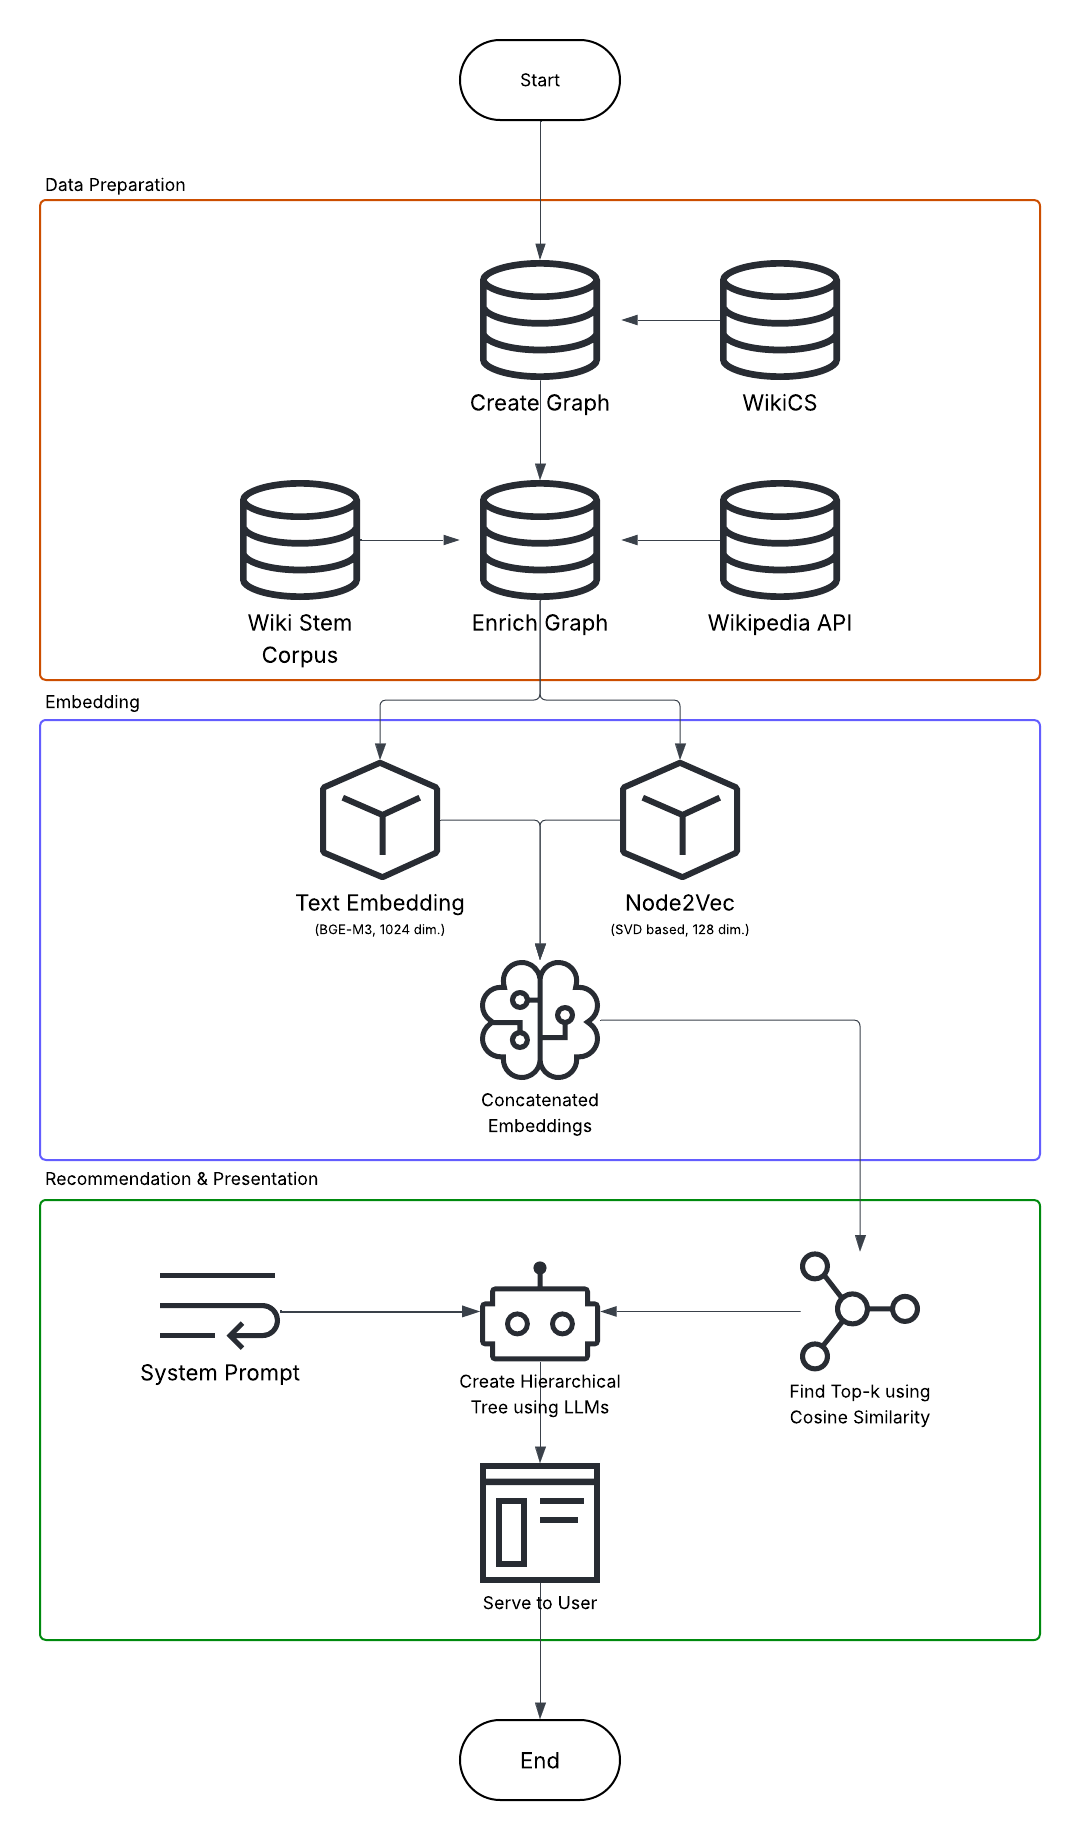
\includegraphics[width=0.88\textwidth]{figures/architecture.png}
\caption{Architecture conceptuelle du pipeline du projet, de la création du graphe jusqu'à la recommandation et à une future présentation en parcours d'apprentissage. La figure reflète la direction générale visée plutôt que chaque détail de l'implémentation courante du prototype.}
\label{fig:architecture}
\end{figure}

Le projet comprend également un prototype interactif destiné à l'utilisateur.
L'application web actuelle prend en charge la recherche d'articles en direct,
la sélection du modèle, la récupération ordonnée des résultats, la
prévisualisation d'article ainsi qu'une vue expérimentale de parcours
d'apprentissage. Contrairement à la phase antérieure de conception, ce rapport
peut désormais montrer l'interface effectivement implémentée et non plus
seulement une maquette. La vue de récupération ordonnée illustrée en
Figure~\ref{fig:ui-ranked} montre la disposition actuelle en trois panneaux :
recherche et sélection du modèle à gauche, sortie de recommandation au centre,
et détail de l'article à droite. L'interface est déjà connectée à la branche
révisée eval-3 et expose la famille actuelle de dix modèles.

\begin{figure}[H]
\centering
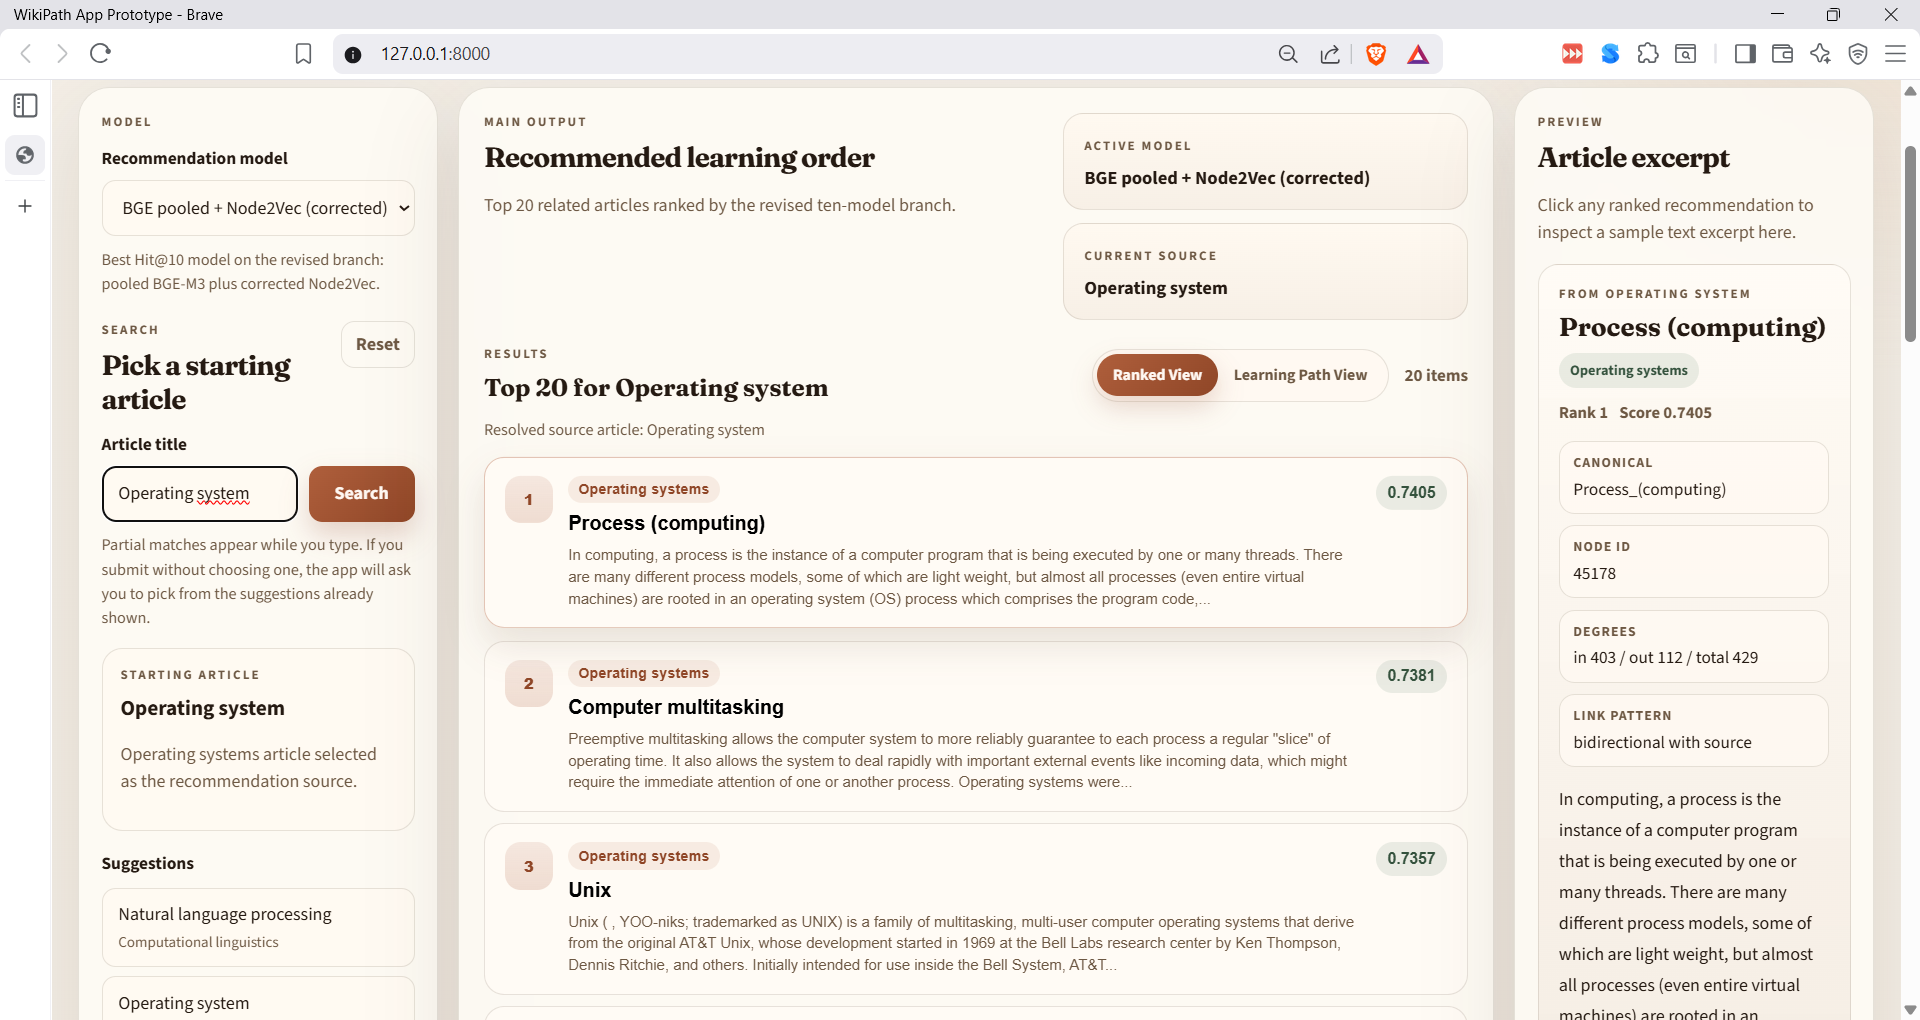
\includegraphics[width=\textwidth]{figures/UI/query-and-results.png}
\caption{Interface implémentée en vue ordonnée du prototype local WikiPath. L'application prend en charge la recherche d'articles, la sélection réelle du modèle, la récupération des 20 meilleurs résultats et une prévisualisation contextuelle.}
\label{fig:ui-ranked}
\end{figure}

La Figure~\ref{fig:ui-models} montre en outre que le prototype implémenté n'est
pas câblé autour d'une seule stratégie de recommandation. L'interface expose
l'ensemble de la famille de modèles révisée, ce qui permet une comparaison
qualitative directe entre les alternatives sémantiques, structurelles,
hybrides, équilibrées par pooling et fondées sur les GNN.

\begin{figure}[H]
\centering
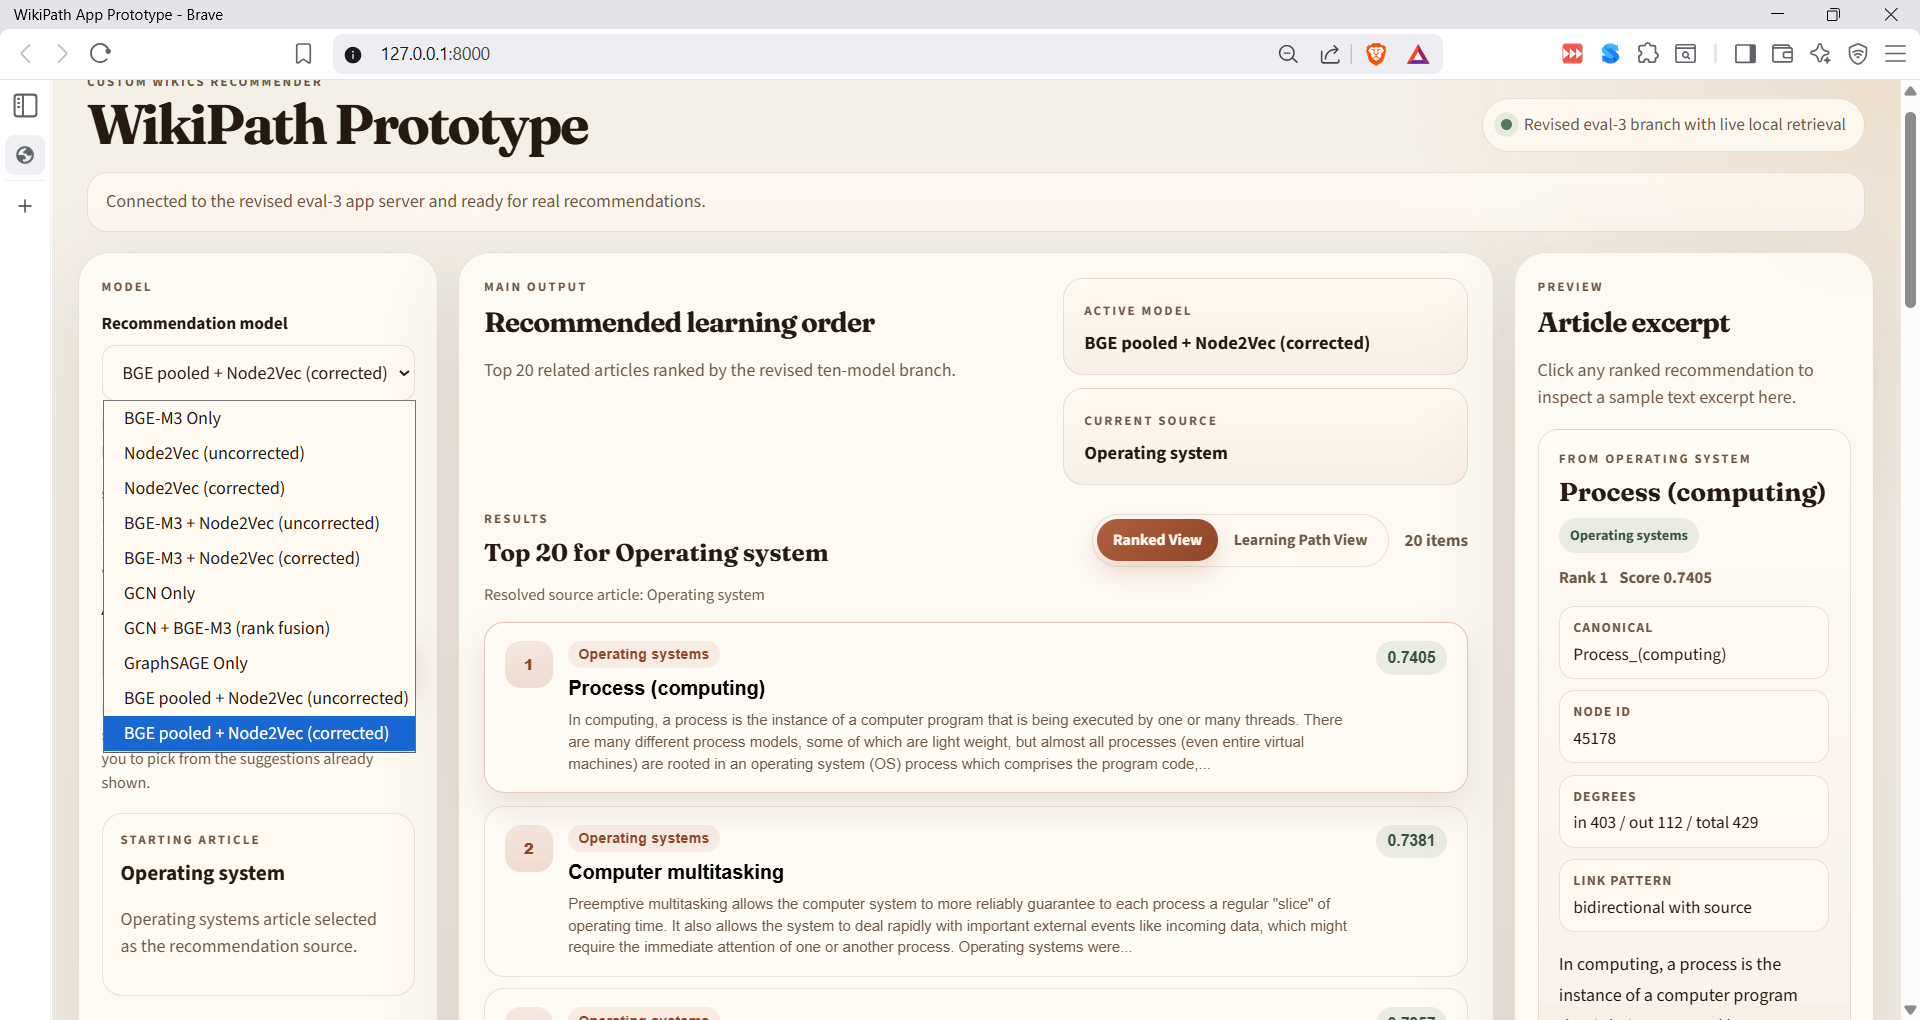
\includegraphics[width=\textwidth]{figures/UI/model-selection.png}
\caption{Panneau de sélection de modèles du prototype implémenté. L'interface expose la famille de modèles issue de l'évaluation révisée, et non un unique recommandateur fixe.}
\label{fig:ui-models}
\end{figure}

Le même prototype contient aussi un mode expérimental de parcours
d'apprentissage illustré en Figure~\ref{fig:ui-path}. Dans ce mode, les
articles les mieux classés sont réorganisés en sections telles que
fondations, concepts centraux, sujets avancés et sujets adjacents. Cette
partie de l'application doit encore être comprise comme une couche
exploratoire d'interface plutôt que comme un produit finalisé de
recommandation, mais elle montre déjà comment une liste ordonnée plate peut
être transformée en une présentation plus orientée vers l'apprentissage.

\begin{figure}[H]
\centering
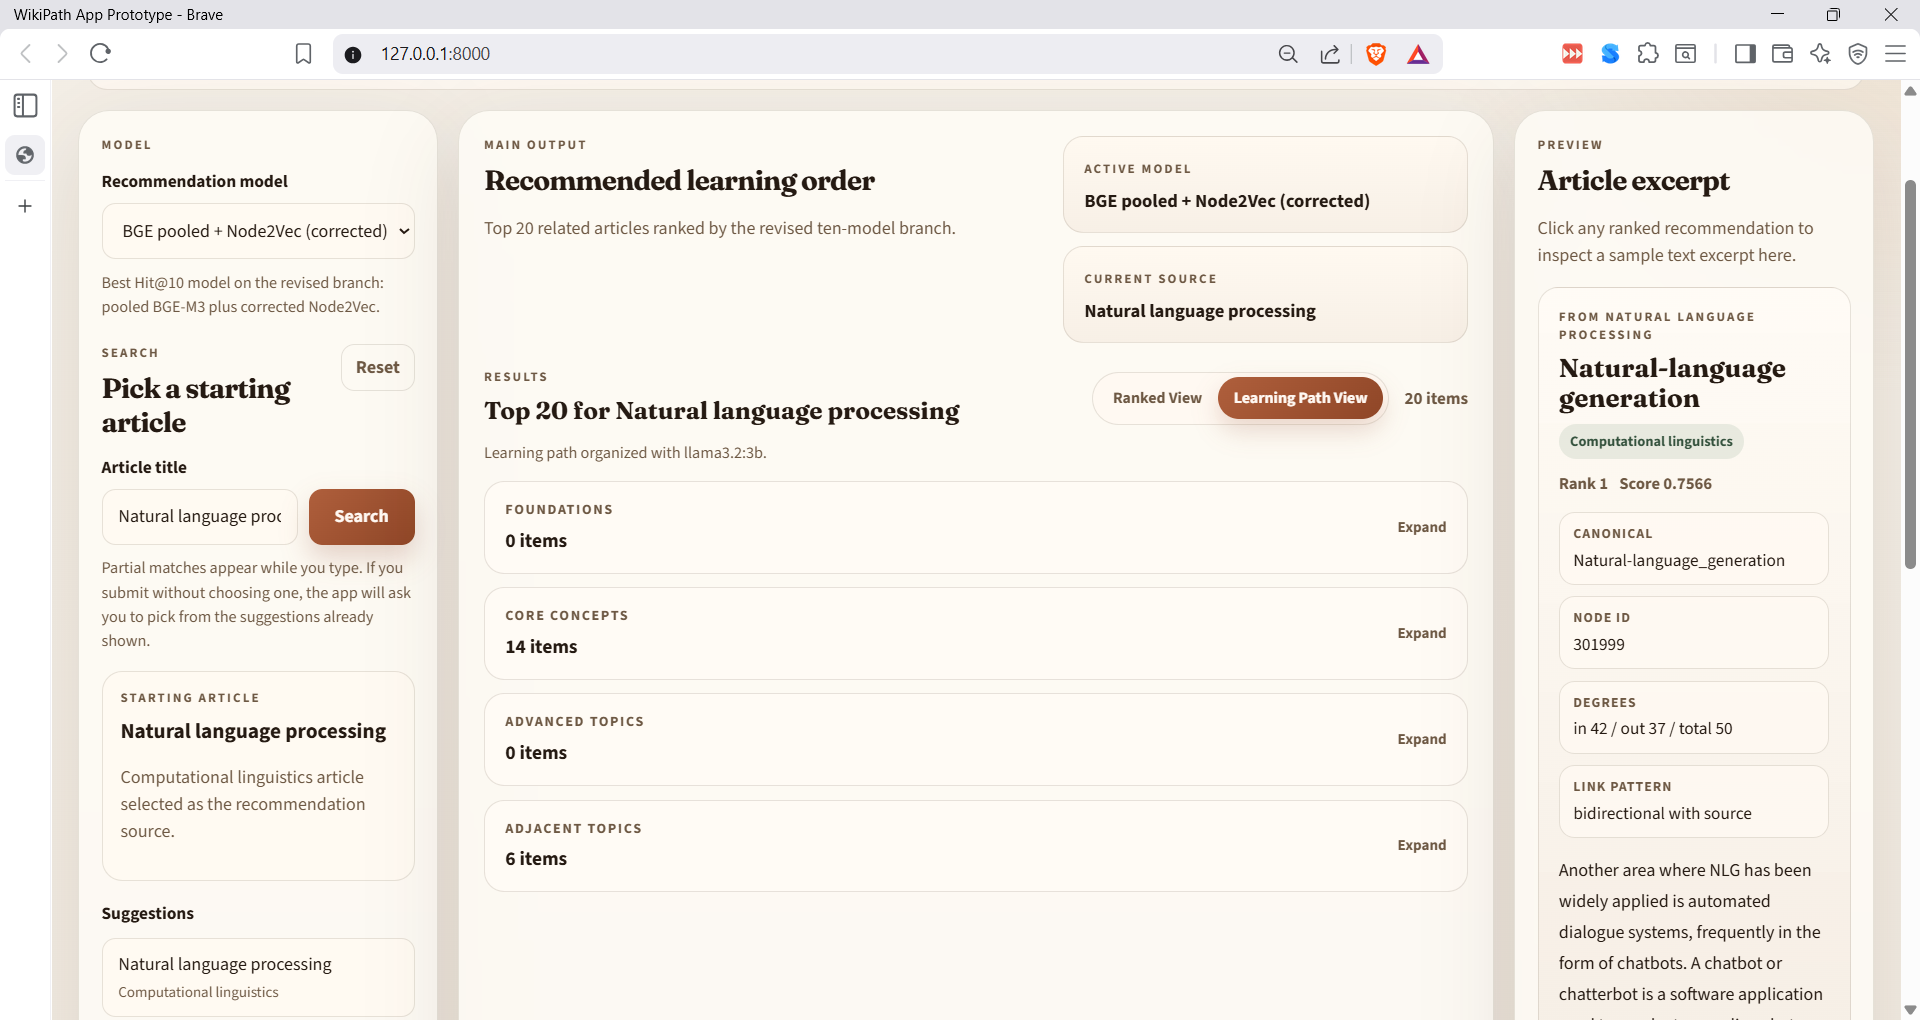
\includegraphics[width=\textwidth]{figures/UI/path-result.png}
\caption{Vue expérimentale de parcours d'apprentissage du prototype. L'ensemble recommandé et ordonné est réorganisé en groupes sectionnés pour une présentation davantage centrée sur le lecteur.}
\label{fig:ui-path}
\end{figure}

À l'heure actuelle, cette vue de parcours d'apprentissage est pilotée par un
petit LLM local via Ollama plutôt que par un grand modèle hébergé. Cela
maintient le prototype entièrement local et praticable sur un matériel
ordinaire, mais signifie aussi que la qualité de l'organisation du parcours est
plus variable que celle de la récupération ordonnée. L'implémentation actuelle
est donc utile comme prototype du schéma d'interaction, tandis que la qualité
sous-jacente de génération du parcours nécessite encore des améliorations.

Les résultats de l'analyse structurelle issus des étapes antérieures restent
également pertinents. La distribution de degré du graphe continue à présenter
un comportement à queue lourde, ce qui a motivé les expériences de correction
sensibles à la popularité ensuite utilisées dans la famille Node2Vec. Cela est
de nouveau illustré en Figure~\ref{fig:degree-log-log}.

\begin{figure}[H]
\centering
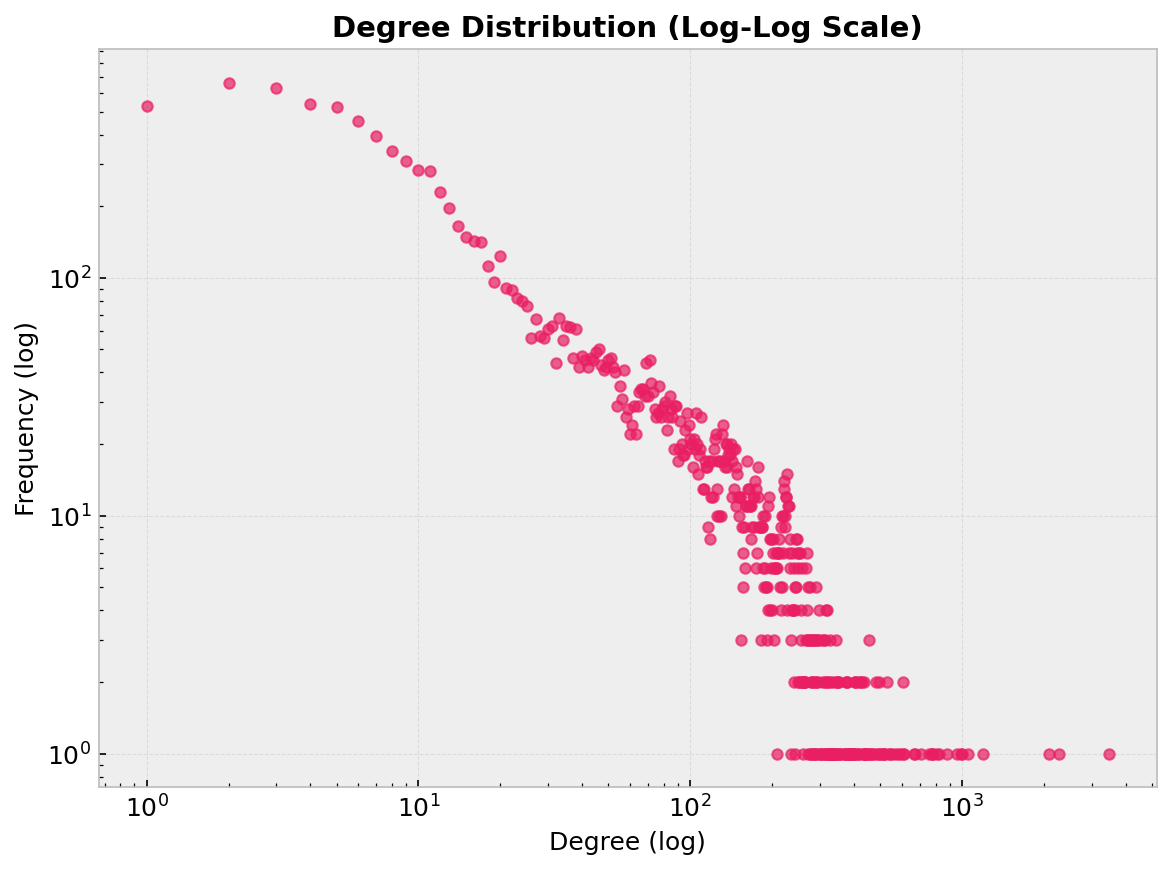
\includegraphics[width=0.78\textwidth]{figures/degree-log-log.png}
\caption{Distribution des degrés en échelle log-log du graphe Custom-WikiCS, montrant le comportement structurel à queue lourde du réseau d'articles.}
\label{fig:degree-log-log}
\end{figure}

Au-delà du seul degré, l'analyse du graphe a aussi montré que l'importance des
nœuds est très inégalement répartie selon les différentes familles de
centralité. La Figure~\ref{fig:centrality} confirme que le degré, le PageRank,
la centralité d'intermédiarité et la centralité de vecteur propre sont tous
fortement asymétriques, ce qui renforce la nécessité de surveiller les effets
de popularité dans les expériences de recommandation.

\begin{figure}[H]
\centering
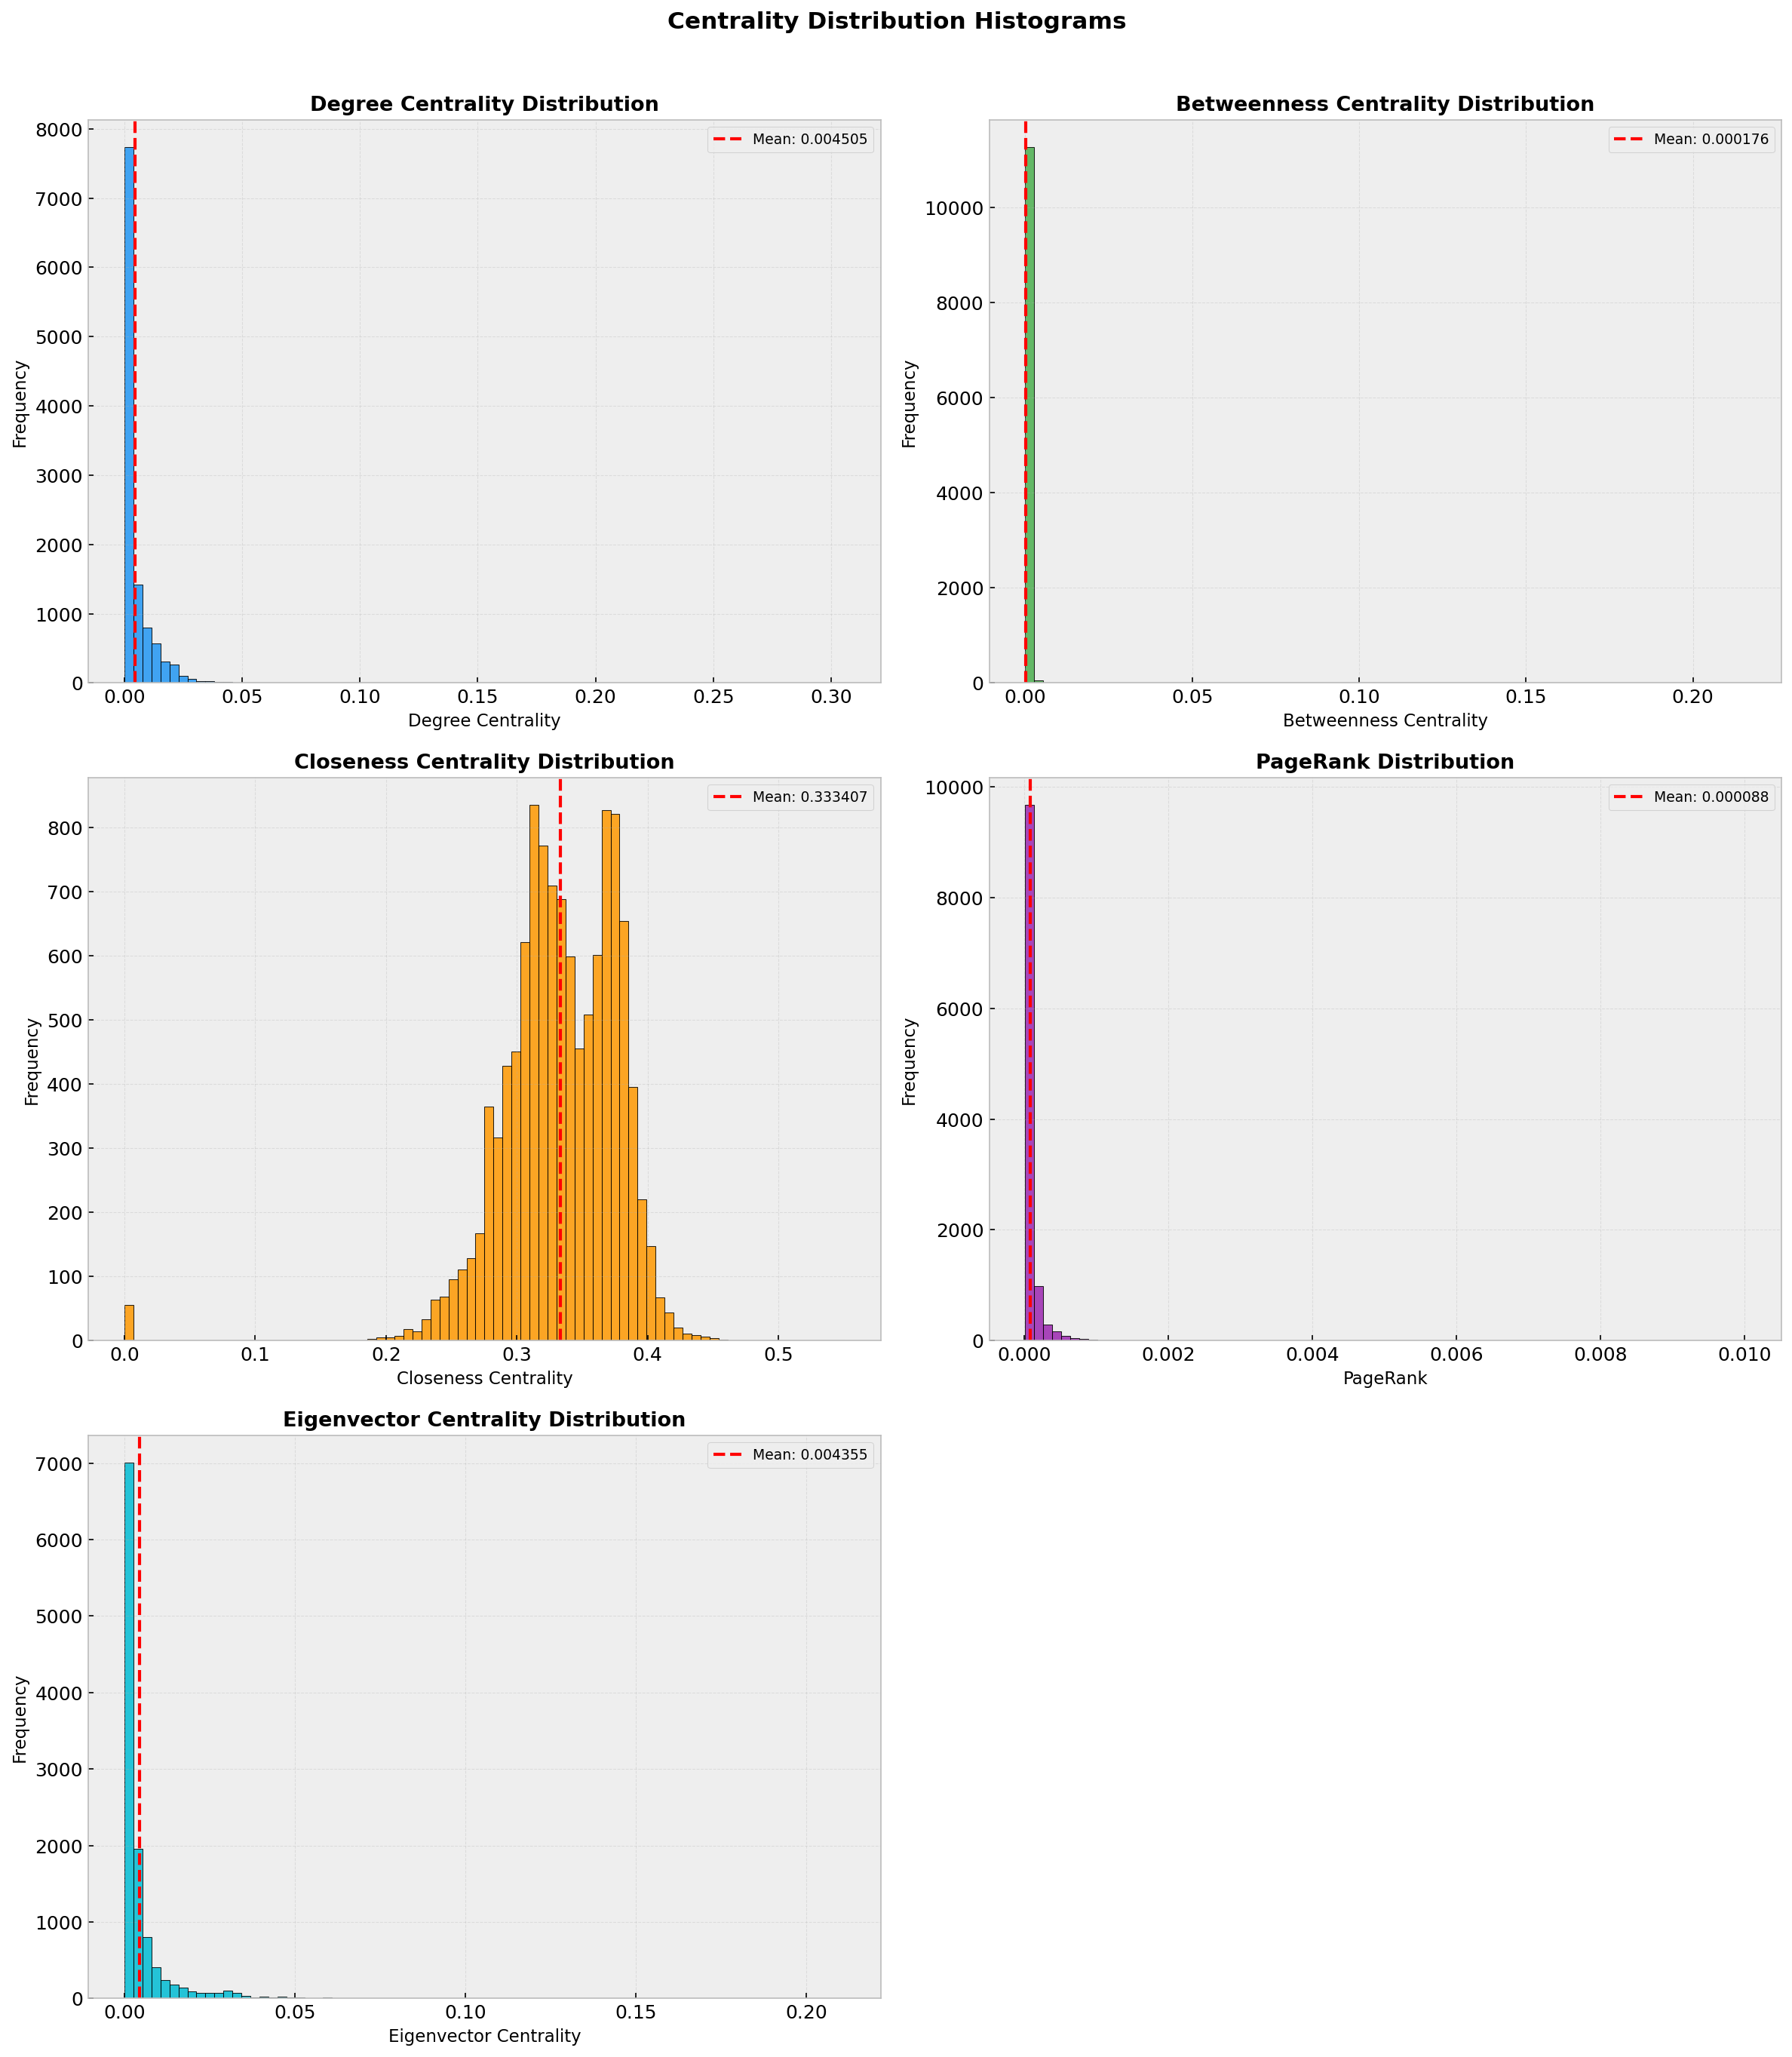
\includegraphics[width=0.88\textwidth]{figures/centrality-histograms.png}
\caption{Histogrammes de distribution des centralités issus de l'analyse du graphe Custom-WikiCS. La forte asymétrie observée pour plusieurs mesures de centralité motive une évaluation sensible à la popularité.}
\label{fig:centrality}
\end{figure}

L'analyse des communautés a également produit un résultat structurel
significatif. La partition de Louvain présentée en Figure~\ref{fig:louvain}
indique que le graphe n'est pas uniformément mélangé, mais organisé en
communautés de tailles très inégales. Cela soutient l'idée qu'un modèle de
recommandation doit équilibrer les voisinages thématiques locaux avec la
connectivité plus globale du graphe.

\begin{figure}[H]
\centering
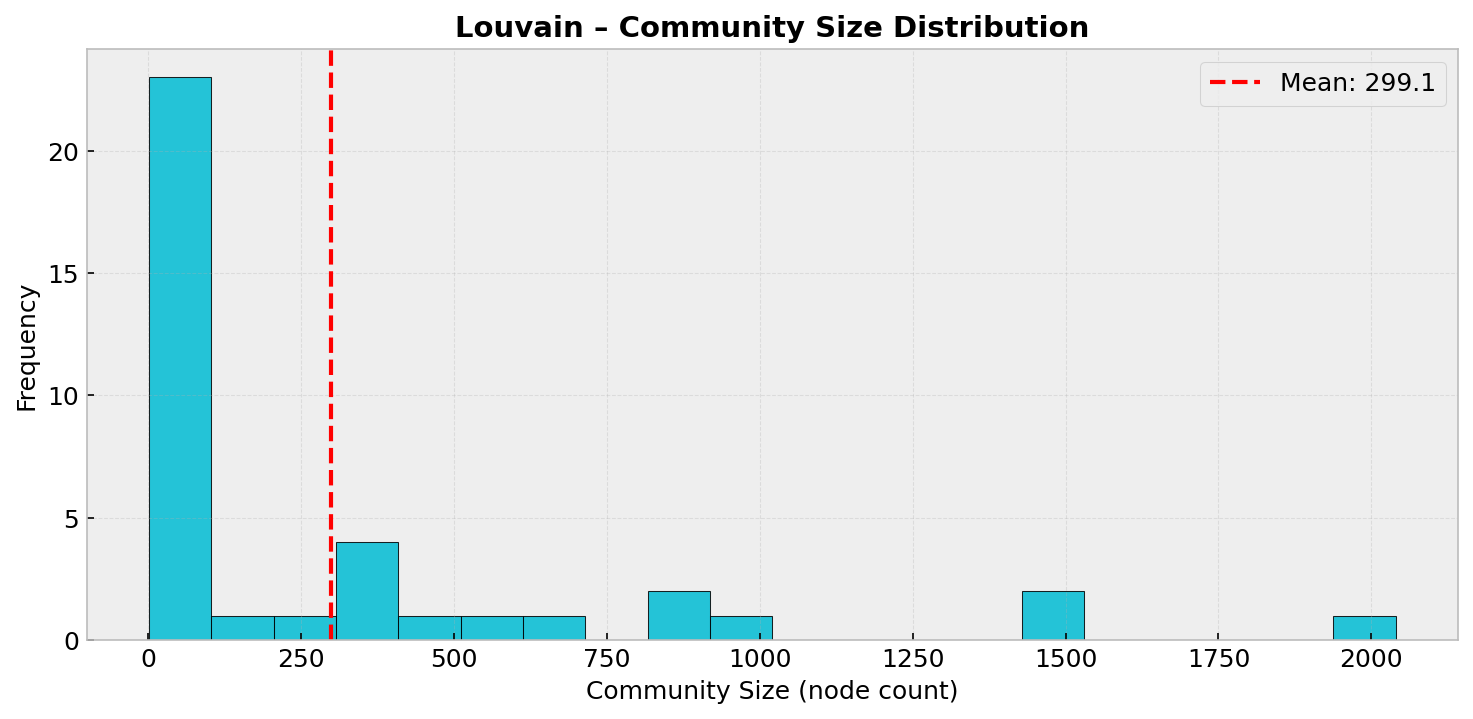
\includegraphics[width=0.82\textwidth]{figures/community-size-distribution-louvain.png}
\caption{Distribution des tailles de communautés de Louvain pour le graphe Custom-WikiCS. Quelques grandes communautés coexistent avec de nombreuses petites, ce qui indique une structure thématique non uniforme.}
\label{fig:louvain}
\end{figure}

\section{Résultats expérimentaux actuels}

Le résultat le plus important à ce stade est la branche d'évaluation révisée
construite sur une séparation structurelle non orientée. Dans cette branche,
le graphe complet est d'abord converti en graphe non orienté, puis séparé en
172\,900 arêtes d'entraînement et 43\,223 arêtes de test, produisant
86\,446 paires d'évaluation étendues sur 9\,022 nœuds d'évaluation. Cette
branche réentraîne la famille structurelle et évalue dix modèles au sein d'une
comparaison unique.

Le Tableau~\ref{tab:selected-results} présente un résumé compact des résultats
actuels. Les meilleures performances proviennent désormais de la famille
hybride corrigée, et non plus uniquement d'une récupération structurelle pure.

\begin{table}[H]
\centering
\caption{Résultats sélectionnés de la branche d'évaluation révisée à dix modèles.}
\label{tab:selected-results}
\begin{tabular}{p{0.38\textwidth}cccc}
\toprule
\textbf{Modèle} & \textbf{Hit@10} & \textbf{MRR} & \textbf{Pop. Lift} & \textbf{ILD} \\
\midrule
BGE pooled + Node2Vec (corrected) & 0.0867 & 0.0410 & 1.3301 & 0.4372 \\
BGE-M3 + Node2Vec (corrected) & 0.0867 & 0.0421 & 1.3081 & 0.4316 \\
Node2Vec (uncorrected) & 0.0781 & 0.0375 & 1.3374 & 0.4569 \\
Node2Vec (corrected) & 0.0781 & 0.0375 & 1.3374 & 0.4569 \\
GCN + BGE-M3 (rank fusion) & 0.0763 & 0.0335 & 1.6650 & 0.4366 \\
BGE-M3 Only & 0.0757 & 0.0366 & 1.9413 & 0.3713 \\
GCN Only & 0.0346 & 0.0180 & 1.1879 & 0.5135 \\
GraphSAGE Only & 0.0122 & 0.0076 & 1.3134 & 0.5313 \\
\bottomrule
\end{tabular}
\end{table}

Ces résultats suggèrent déjà deux conclusions importantes. Premièrement,
l'impression plus ancienne selon laquelle le Node2Vec non corrigé dominait
nettement le projet n'est plus valable dans la branche révisée. Deuxièmement,
les modèles les plus performants sont désormais les hybrides
sémantico-structurels, en particulier les variantes corrigées qui combinent
BGE-M3 avec une information structurelle sans fuite. L'interface de sélection
des modèles montrée dans le prototype rend ces alternatives directement
accessibles pendant les tests interactifs, ce qui a également facilité la
comparaison qualitative entre familles de modèles.
